\chapter{Qualification of the Electronics}
\label{chap:II-5-qualification}

  To prepare the DAQ system for the slice test, the electronic components need to be tested and qualified. For the VFAT2s, qualification procedures have to be developed to characterize the analog front-end of each chip, record their response to calibration pulses, and optimize the parameters to achieve uniformity over the entire detector. For the GEB, qualification means ensuring that no shorts are present and that the integrity of the signals is kept over the full length of the board. Finally, the system as a whole needs to be tested against communication errors or readout problems.

  \section{Qualification of the VFAT2s}

    The qualification process of the VFAT2s has been automatized using Python scripts to run the various procedures using the dedicated firmware modules of the OptoHybrid. The aim of this tools is to reject faulty chips and record the parameters of the analog front-end which slightly vary from component to component.

    \subsection{Threshold Scans}

      The first step of the procedure is to run a threshold scan for each channel to reveal those that are not responding or that are noisy. To do so, the tools use the threshold scan module of the firmware that relies on tracking data to perform a scan of each channel. 

      \begin{figure}[h!]
        \centering
        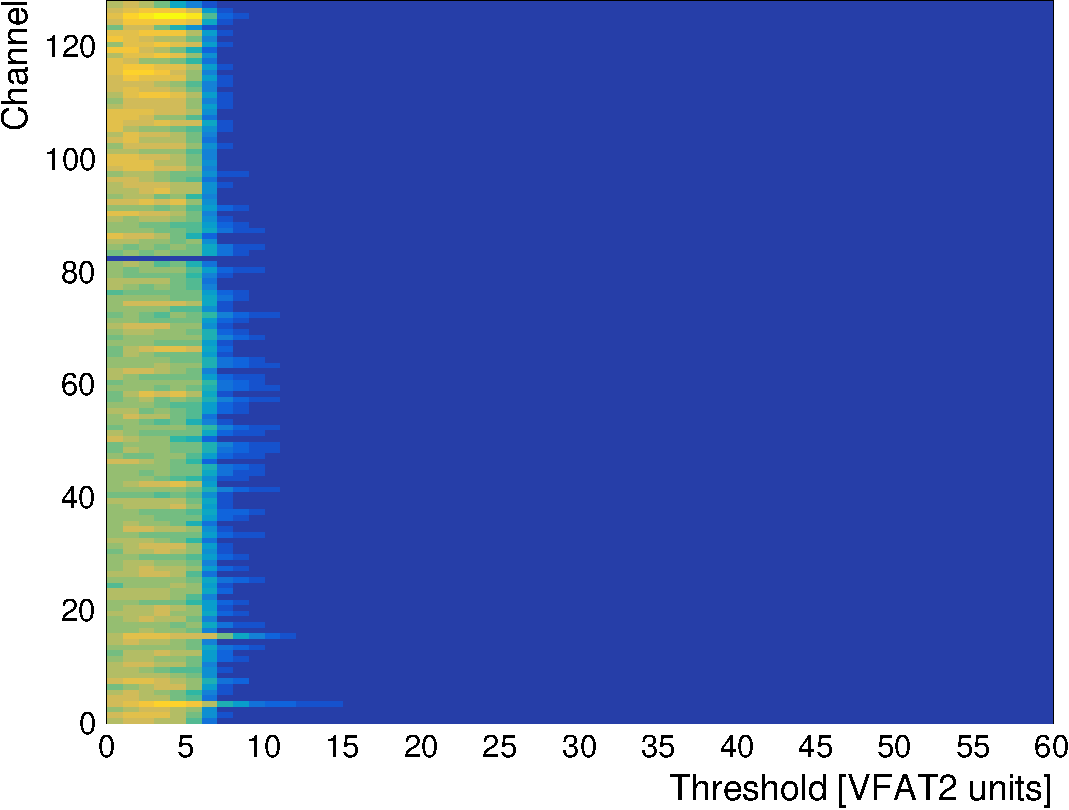
\includegraphics[width=0.5\textwidth]{img/plots/cThreshold_Channel-crop}
        \caption{}
        \label{fig:II-5-qualification-threshold}
      \end{figure}

    \subsection{Front-end Currents and Voltages}

      \begin{figure}[h!]
        \centering
        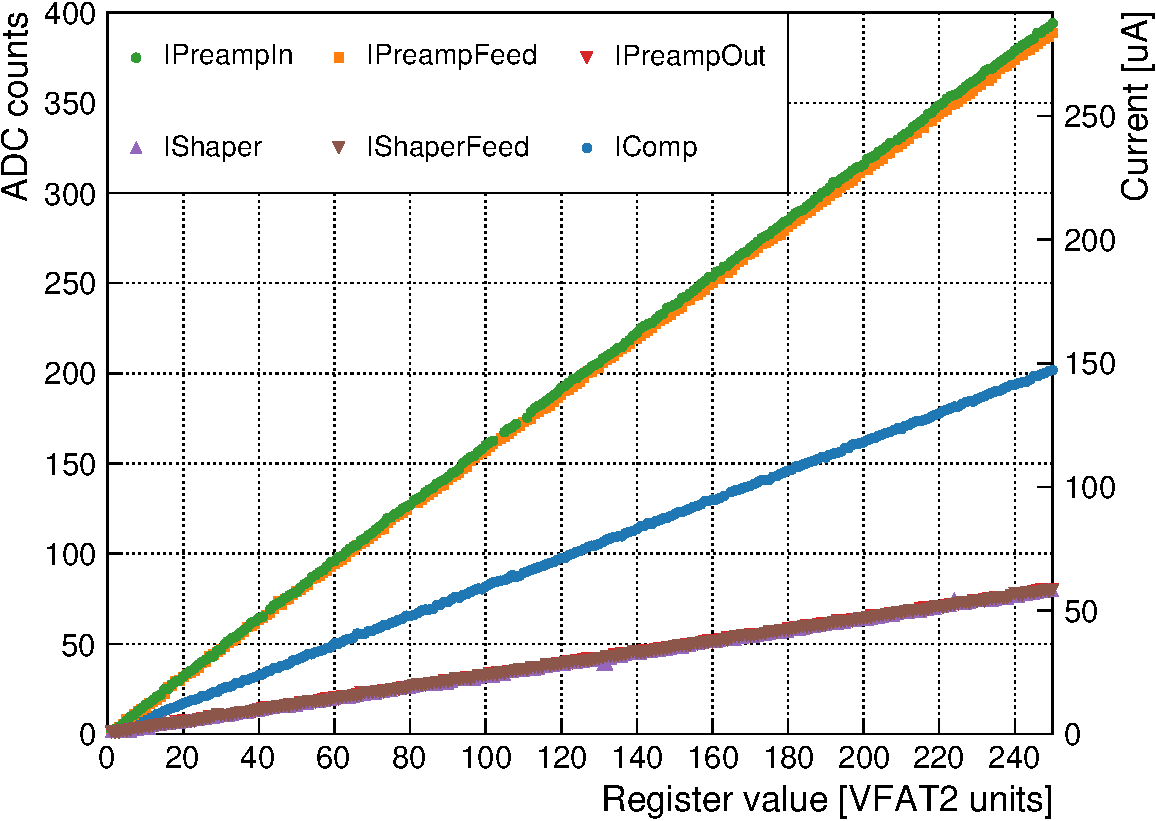
\includegraphics[width=0.49\textwidth]{img/plots/cADC_Current-crop}
        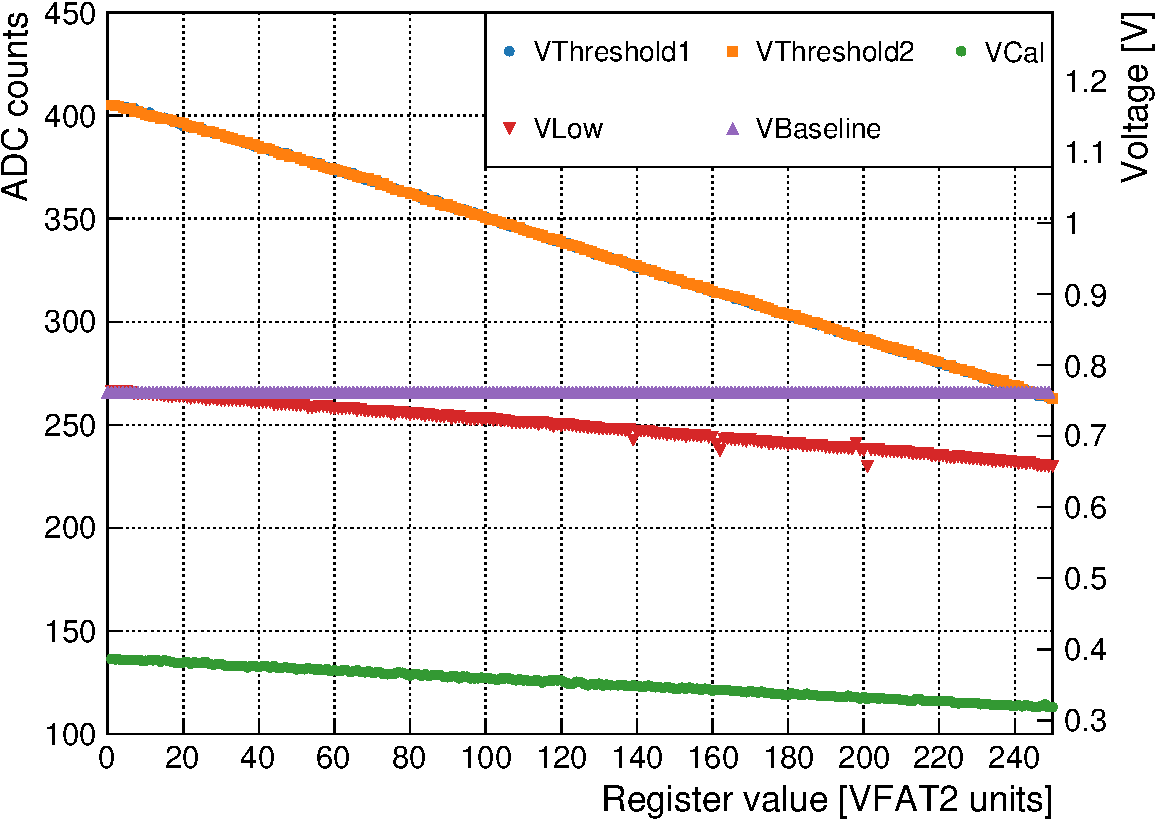
\includegraphics[width=0.49\textwidth]{img/plots/cADC_Voltage-crop}
        \caption{}
        \label{fig:II-5-qualification-adc}
      \end{figure}

    \subsection{S-Curve Scans}

      \begin{figure}[h!]
        \centering
        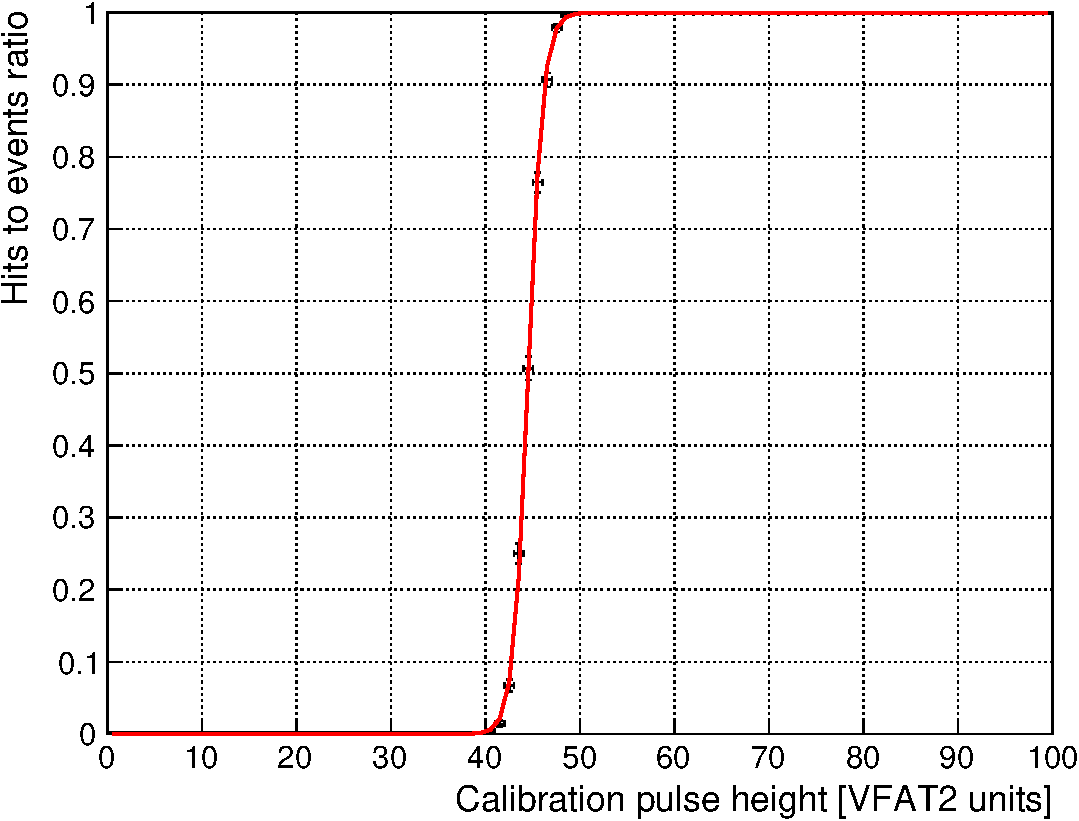
\includegraphics[width=0.5\textwidth]{img/plots/cSCurve_T25-crop}
        \caption{}
        \label{fig:II-5-qualification-scurve}
      \end{figure}

      \begin{figure}[h!]
        \centering
        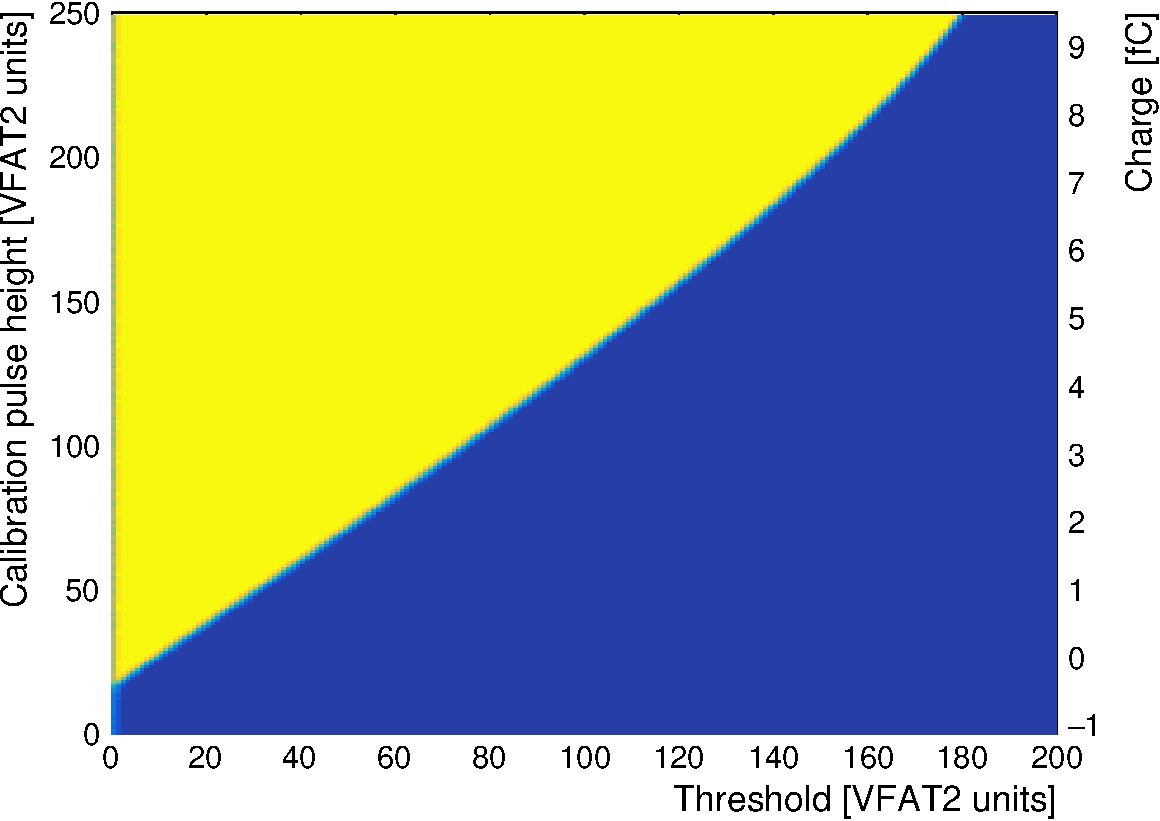
\includegraphics[width=0.49\textwidth]{img/plots/cSCurve_ThresholdVCal-crop}
        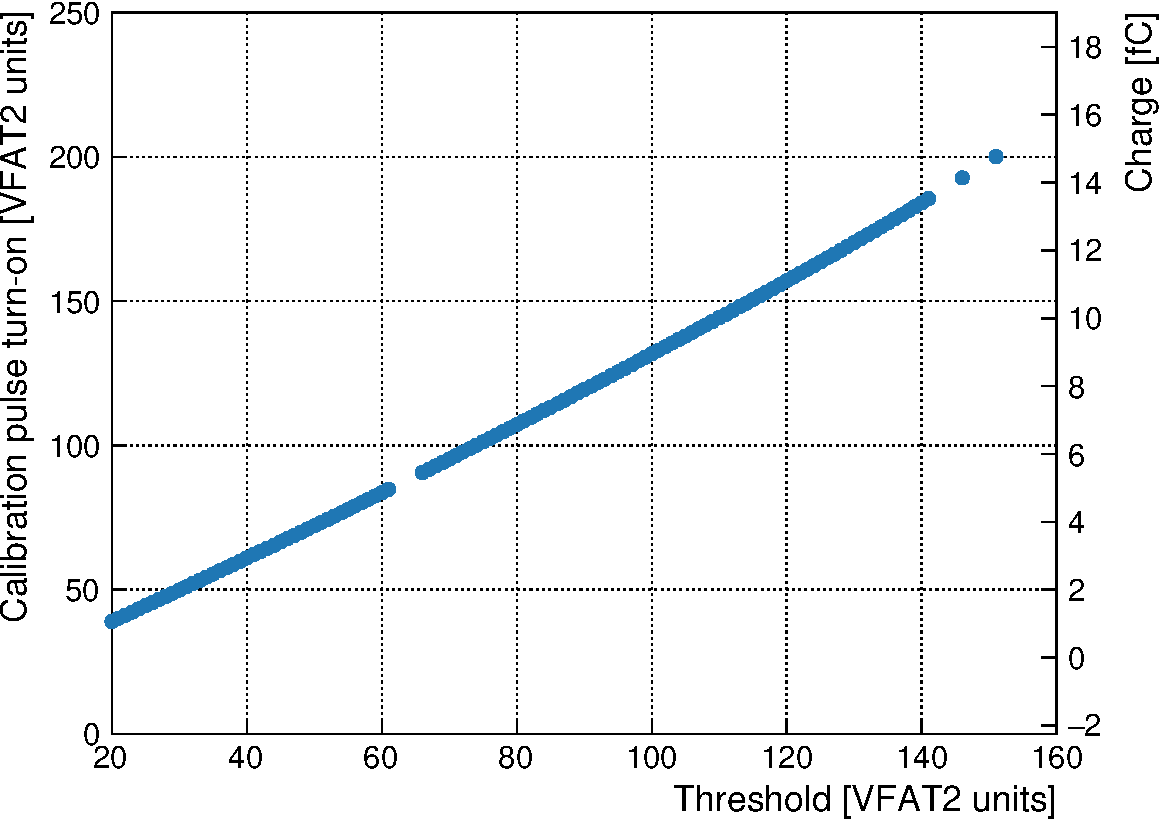
\includegraphics[width=0.49\textwidth]{img/plots/cSCurve_TurnOn-crop}
        \caption{}
        \label{fig:II-5-qualification-scurves}
      \end{figure}

      \begin{figure}[h!]
        \centering
        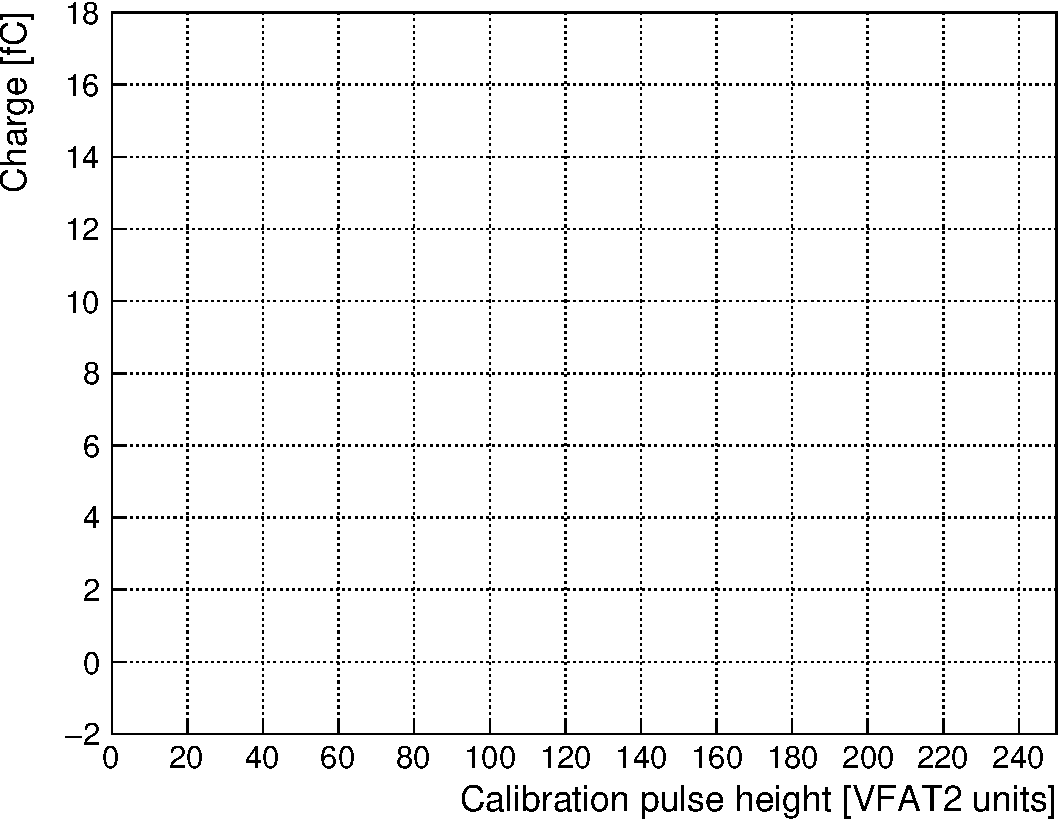
\includegraphics[width=0.5\textwidth]{img/plots/cCal_Charge-crop}
        \caption{}
        \label{fig:II-5-qualification-calcharge}
      \end{figure}

      \begin{figure}[h!]
        \centering
        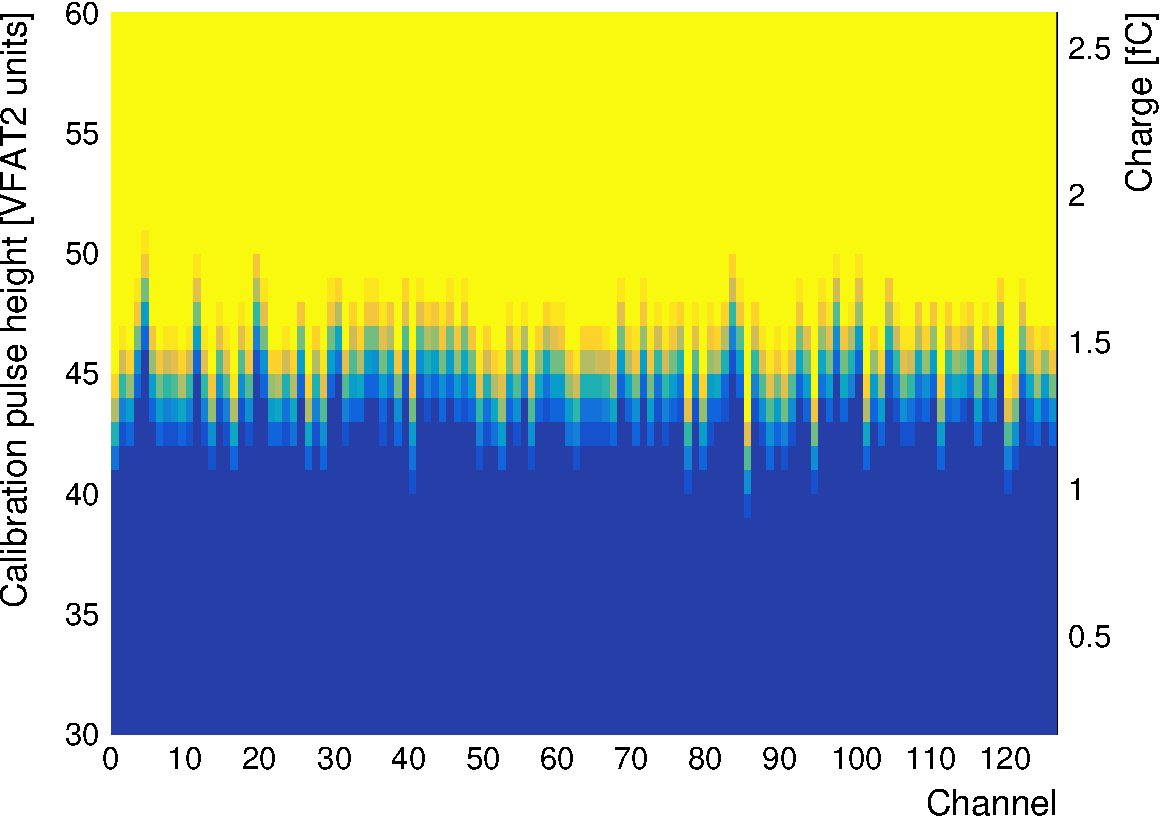
\includegraphics[width=0.49\textwidth]{img/plots/cSCurve_ChannelVCal_Trim0-crop}
        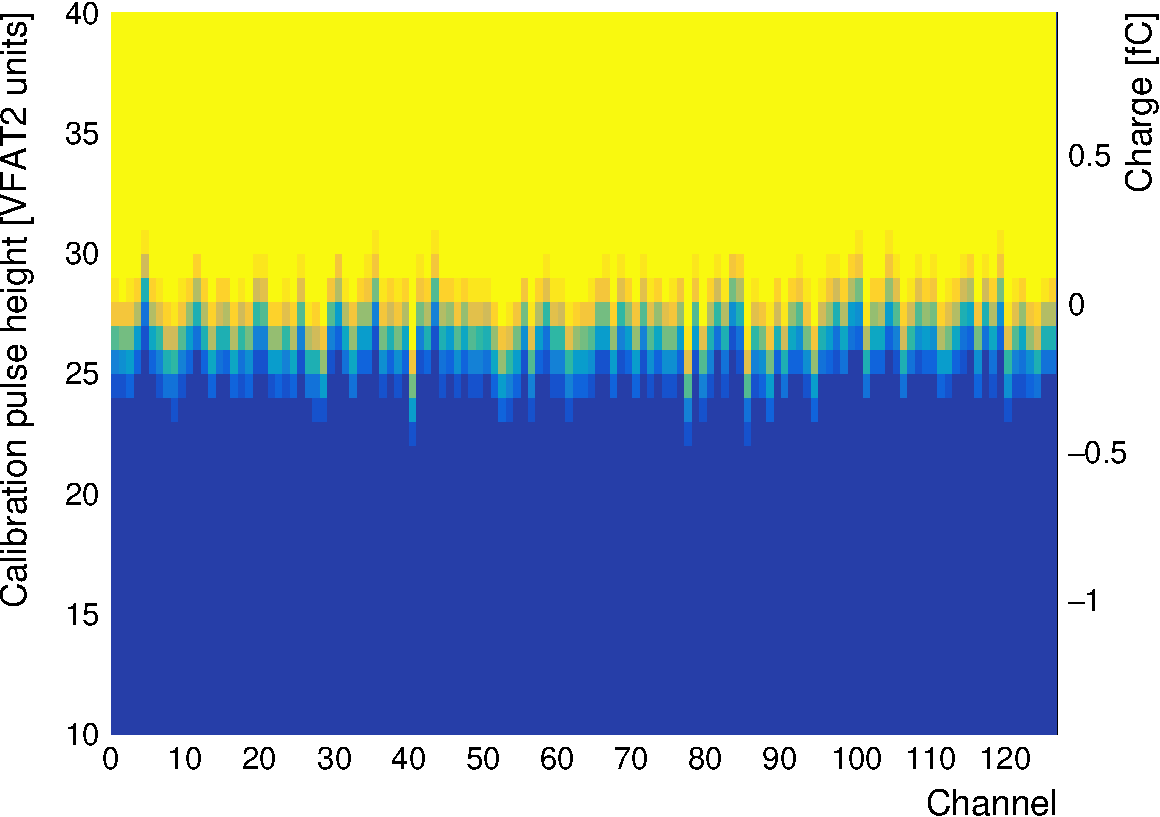
\includegraphics[width=0.49\textwidth]{img/plots/cSCurve_ChannelVCal_Trim1-crop}
        \caption{}
        \label{fig:II-5-qualification-trim}
      \end{figure}

      \begin{figure}[h!]
        \centering
        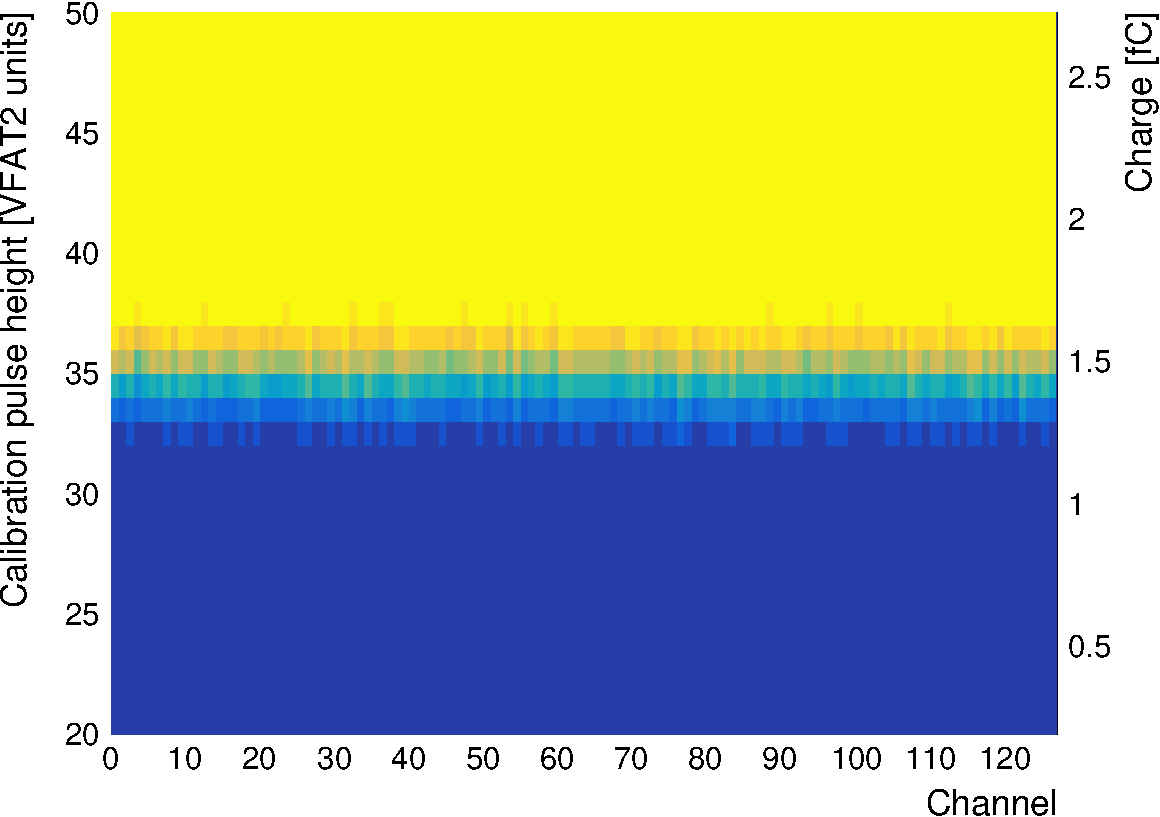
\includegraphics[width=0.49\textwidth]{img/plots/cSCurve_ChannelVCal_Trimed-crop}
        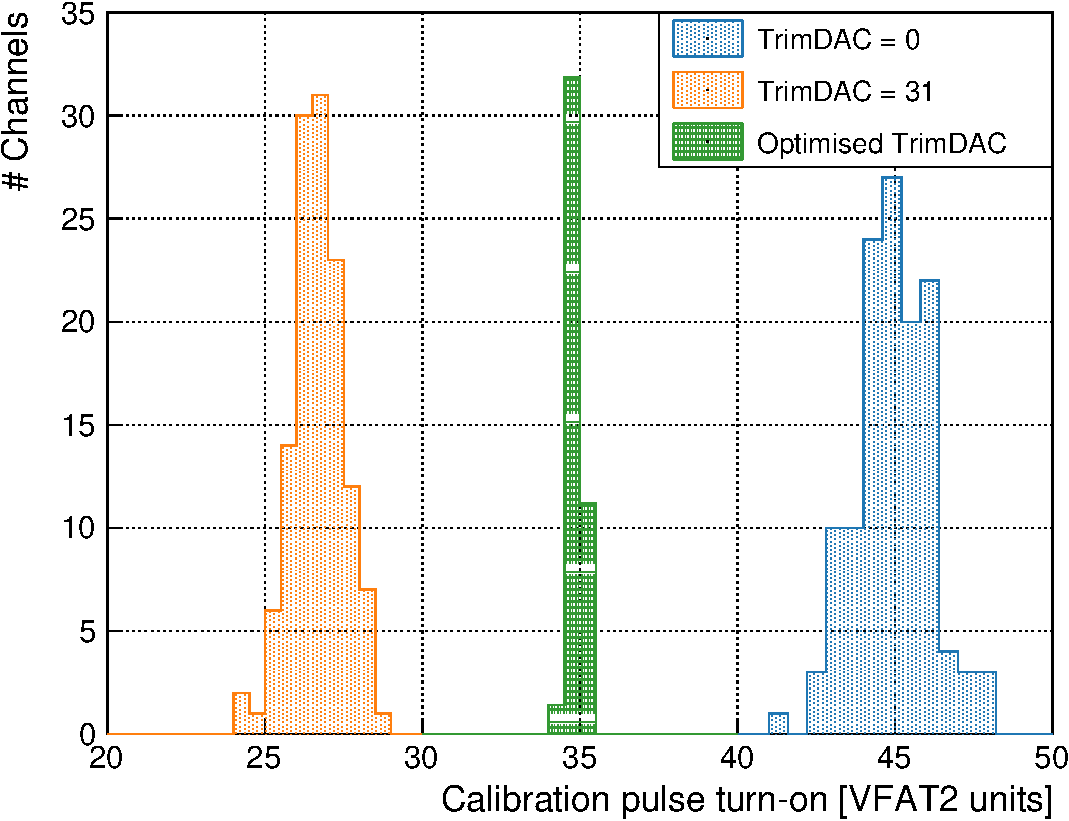
\includegraphics[width=0.49\textwidth]{img/plots/cSCurve_ChannelVCal_Disp-crop}
        \caption{}
        \label{fig:II-5-qualification-trimed}
      \end{figure}



  \section{Qualification of the GEB}

    In order to test the GEB, a small PCB equipped with the same connector as the VFAT2 Hybrids was developed. Using signals originating from the OptoHybrid, the board can check the integrity of the data and use on-board LEDs to signals the results of the tests for the current position.

    \subsection{The GEB Testing Board}

      \begin{figure}[h!]
        \centering
        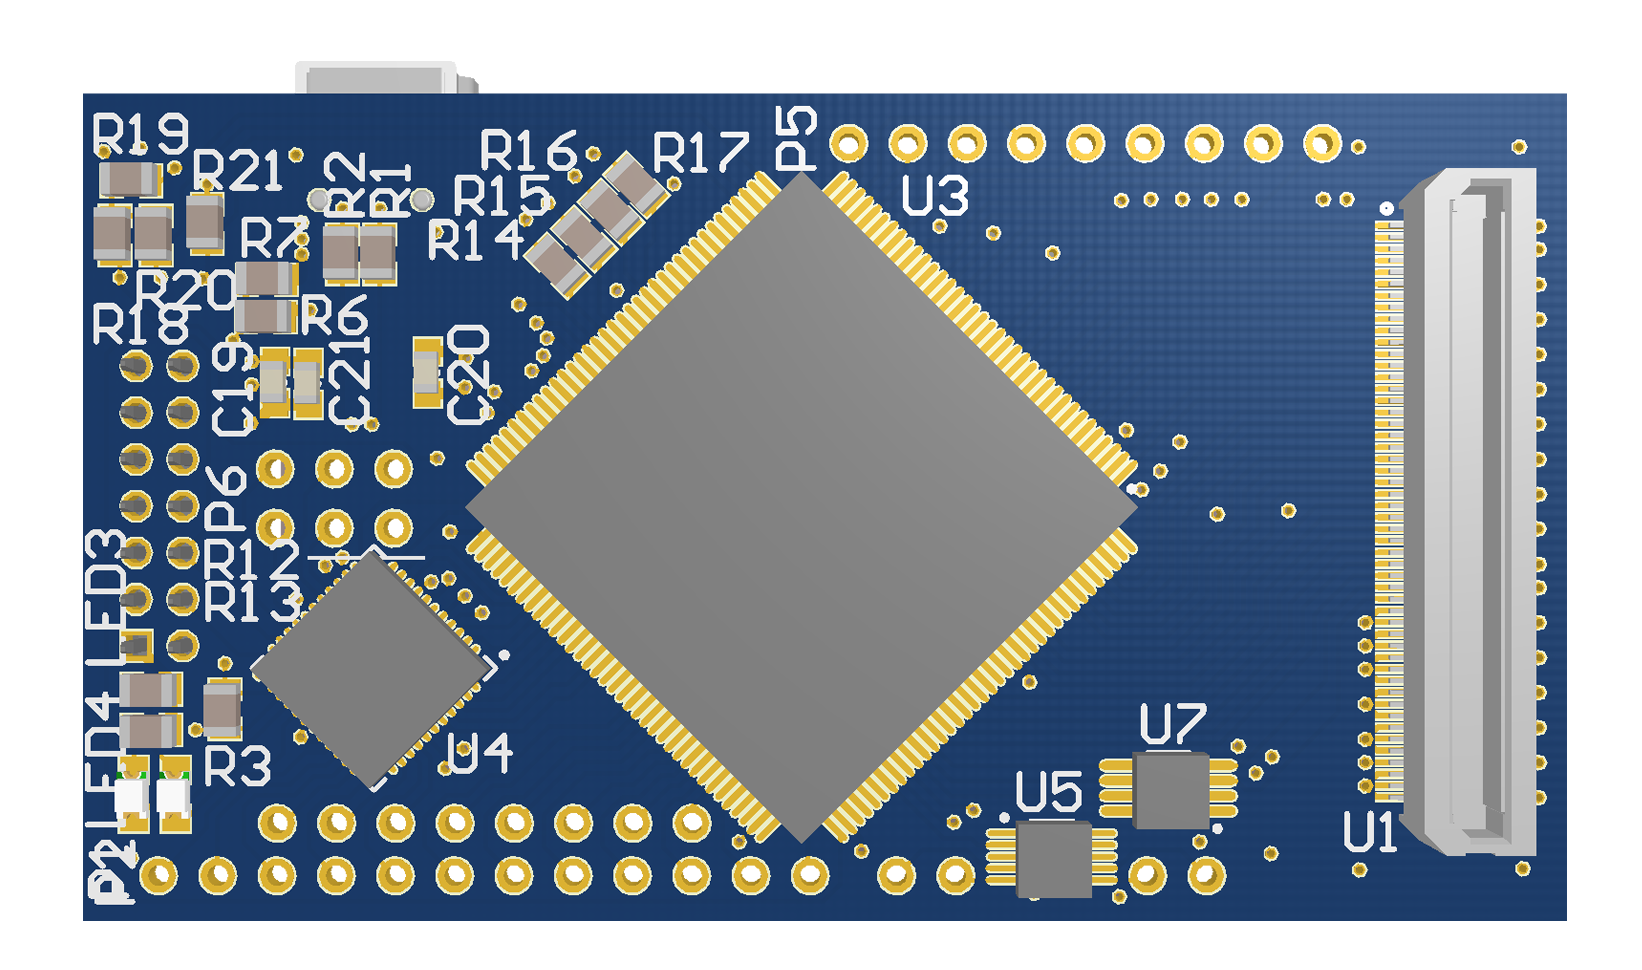
\includegraphics[width=0.49\textwidth]{img/II-5-qualification/geb-3d-0.png}
        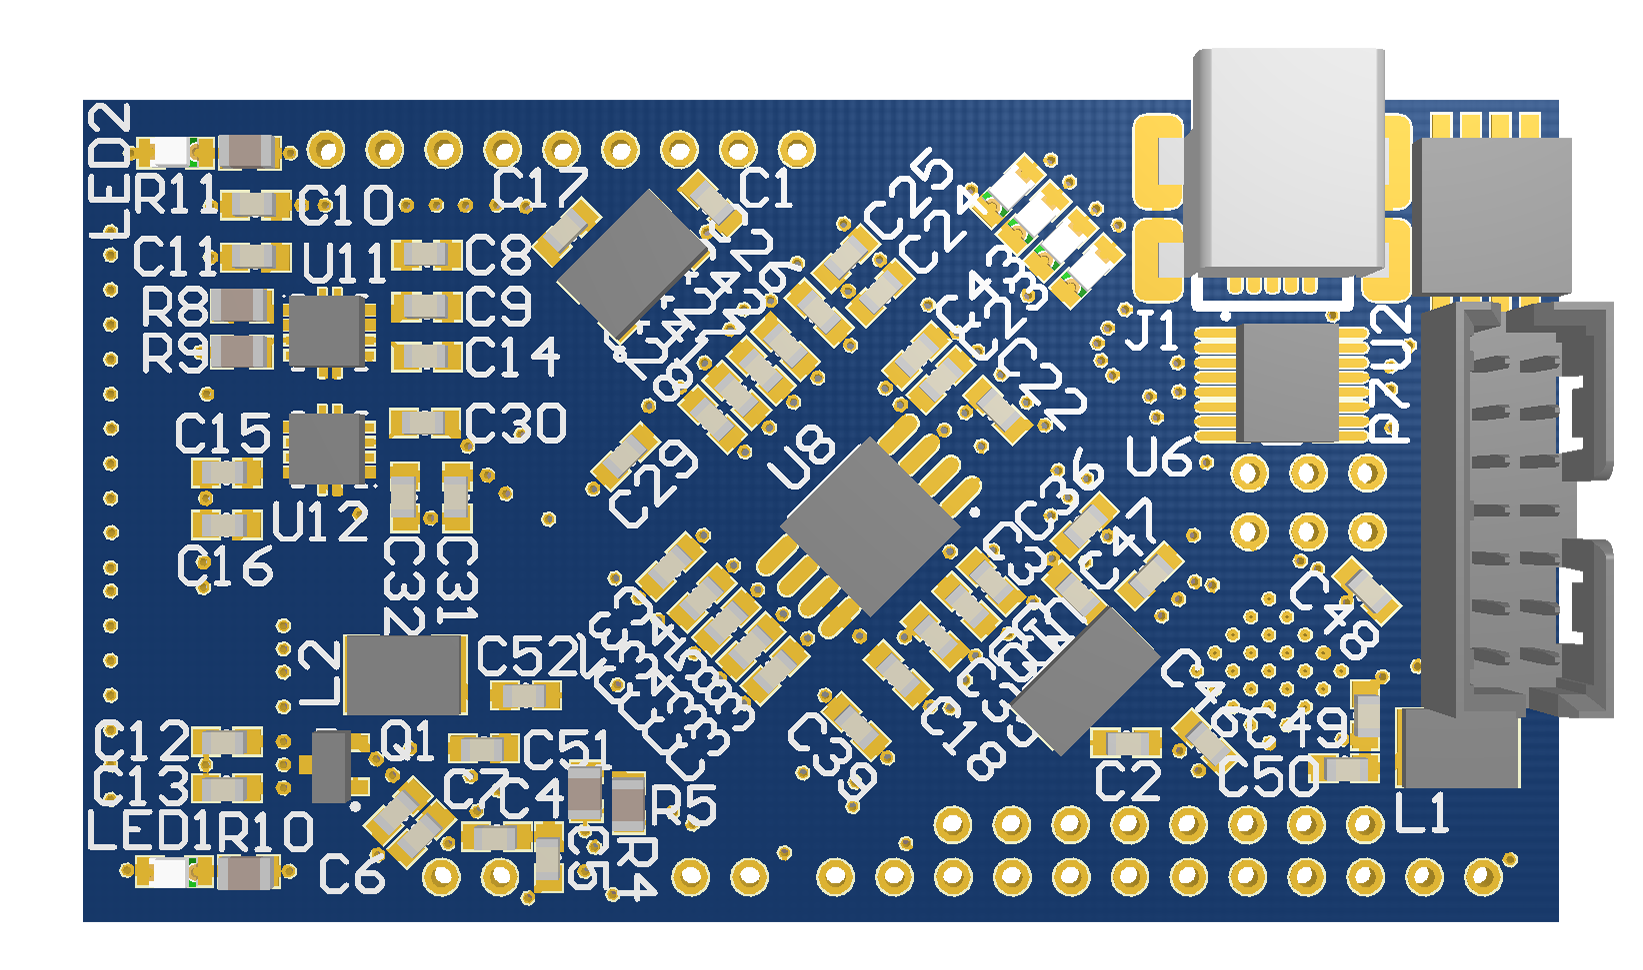
\includegraphics[width=0.49\textwidth]{img/II-5-qualification/geb-3d-1.png}
        \vspace*{0.3cm}
        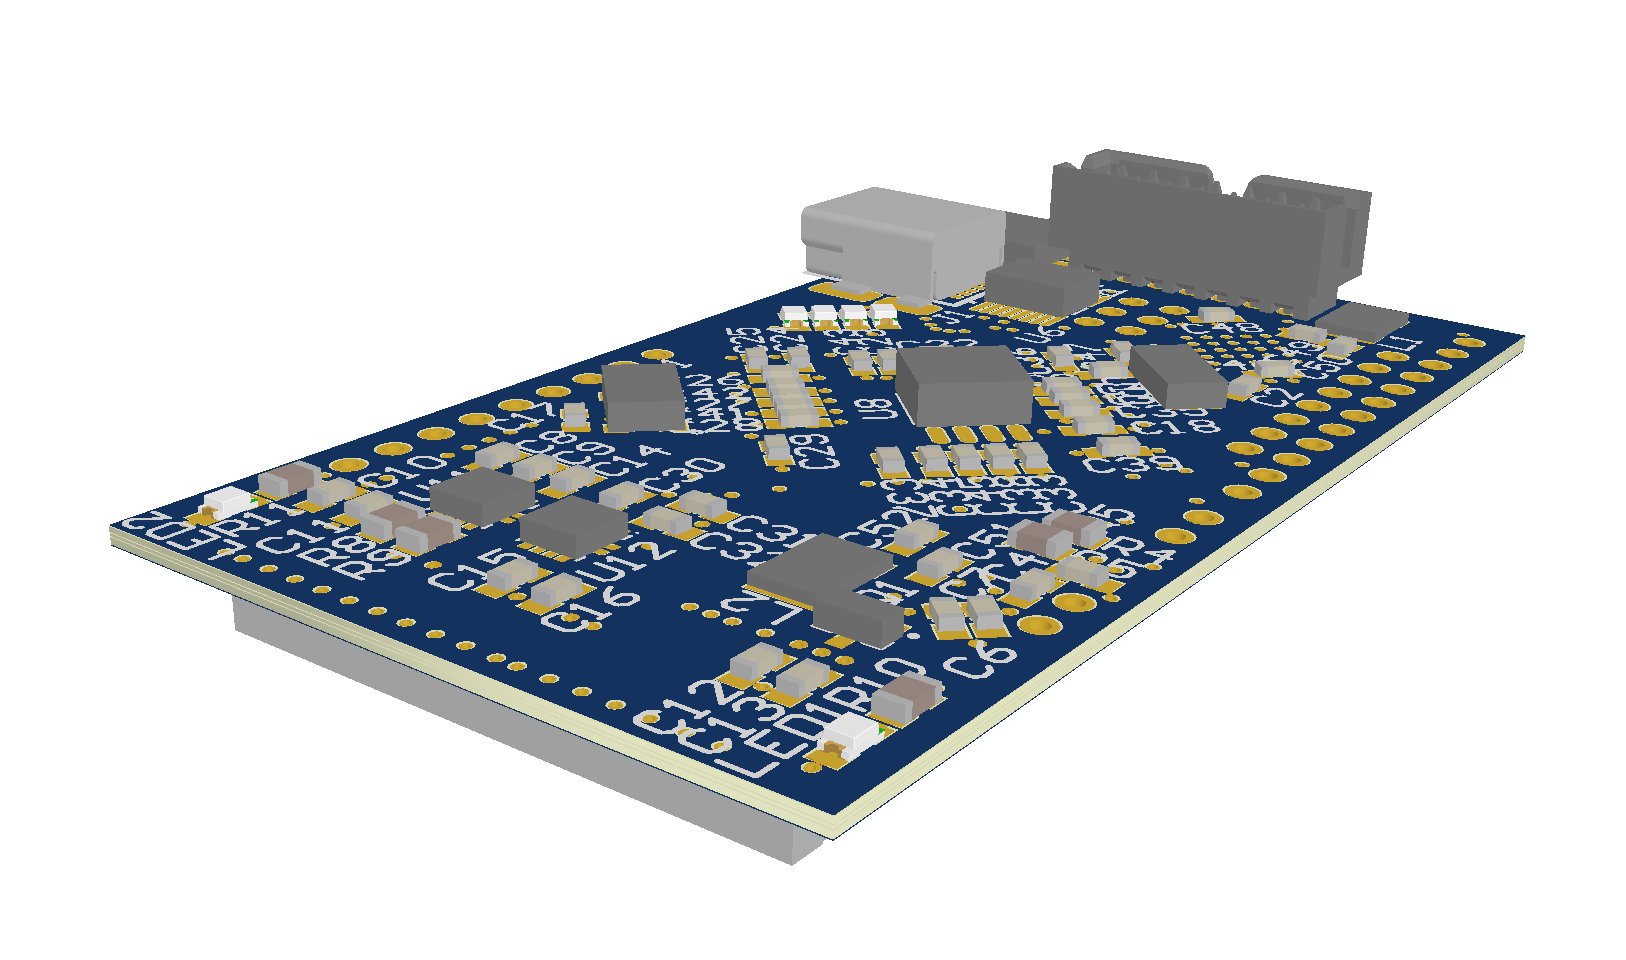
\includegraphics[width=0.49\textwidth]{img/II-5-qualification/geb-3d-2.png}
        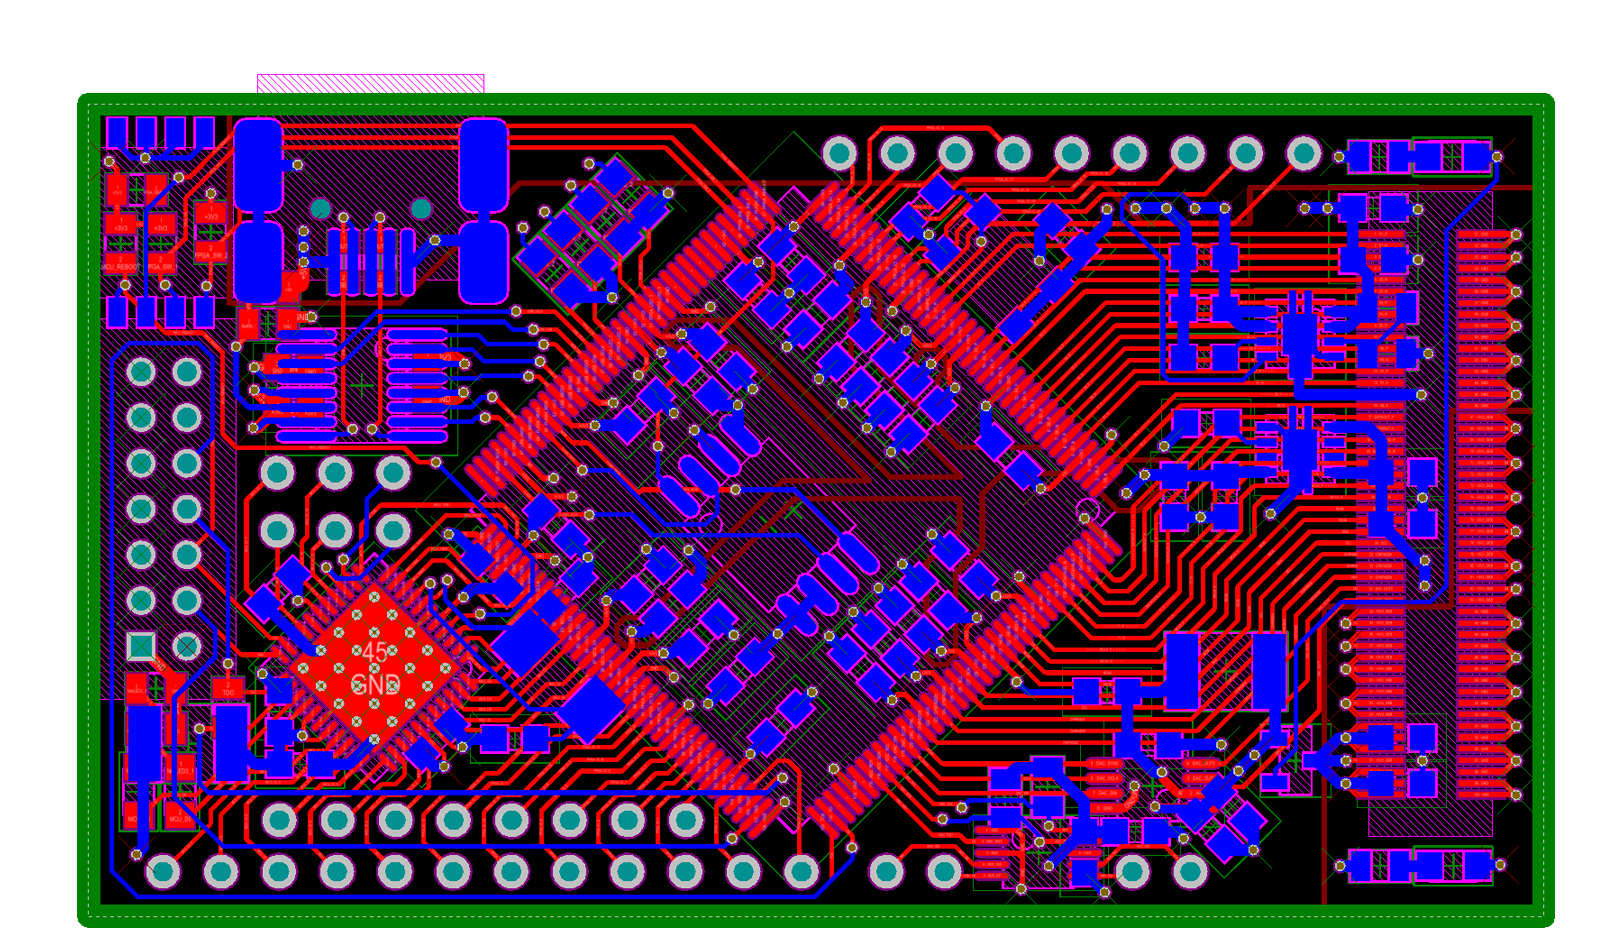
\includegraphics[width=0.49\textwidth]{img/II-5-qualification/geb-pcb.png}
        \caption{}
        \label{fig:II-5-qualification-geb-pcb}
      \end{figure}

  \section{Qualification of the System}

\begin{lstlisting}
A. Testing the GLIB's presence
   Trying to read the GLIB board ID... If this test fails, the script will stop.
   > Passed...

B. Testing the OH's presence
   Trying to set the OptoHybrid registers... If this test fails, the script will stop.
   > Passed...

C. Testing the GLIB registers
   Performing single and FIFO reads on the GLIB counters and ensuring they increment.
   > Passed...

D. Testing the OH registers
   Performing single and FIFO reads on the OptoHybrid counters and ensuring they increment.
   > Passed...

E. Detecting the VFAT2s over I2C
   Detecting VFAT2s on the GEM by reading out their chip ID.
   Detected 18 VFAT2s: [1, 3, 4, 5, 6, 9, 10, 12, 13, 14, 15, 16, 17, 19, 20, 21, 22, 23]

F. Testing the I2C communication with the VFAT2s
   Performing random read/write operation on each connect VFAT2.
   > Passed...  #1
   > Passed...  #3
   > Passed...  #4
   > Passed...  #5
   > Passed...  #6
   > Passed...  #9
   > Passed...  #10
   > Passed...  #12
   > Passed...  #13
   > Passed...  #14
   > Passed...  #15
   > Passed...  #16
   > Passed...  #17
   > Passed...  #19
   > Passed...  #20
   > Passed...  #21
   > Passed...  #22
   > Passed...  #23

G. Reading out tracking data
   Sending triggers and testing if the Event Counter adds up.
   > Passed...  #1
   > Passed...  #3
   > Passed...  #4
   > Passed...  #5
   > Passed...  #6
   > Passed...  #9
   > Passed...  #10
   > Passed...  #12
   > Passed...  #13
   > Passed...  #14
   > Passed...  #15
   > Passed...  #16
   > Passed...  #17
   > Passed...  #19
   > Passed...  #20
   > Passed...  #21
   > Passed...  #22
   > Passed...  #23

H. Reading out tracking data
   Turning on all VFAT2s and looking that all the Event Counters add up.
   > Passed...

I. Testing the tracking data readout rate
   Sending triggers at a given rate and looking at the maximum readout rate that can be achieved.
   Maximum readout rate 175000 Hz

J. Testing the optical link error rate
   GLIB tracking link error rate is of          0 Hz
   GLIB trigger link error rate is of           0 Hz
   OptoHybrid tracking link error rate is of    0 Hz
   OptoHybrid trigger link error rate is of     0 Hz

K. Results
   A.    > Passed...
   B.    > Passed...
   C.    > Passed...
   D.    > Passed...
   E.    > Passed...
   F.    > Passed...
   G.    > Passed...
   H.    > Passed...
   I.    > Passed...
   J.    > Passed...
\end{lstlisting}
